\chapter{Stand der Technik}
% Bezogen auf die eigenen Zielsetzungen und Fragestellungen soll aufgezeigt werden, wie andere
% dieses oder ähnliche Probleme gelöst haben. Worauf können Sie aufbauen, was müssen Sie neu
% angehen? Wodurch unterscheidet sich Ihre Lösung von anderen Lösungen? Für wissenschaftlich
% orientierte Arbeiten sei hier explizit auf (Balzert, S. 66 ff) verwiesen.
In diesem Kapitel werden gängige Technologien vorgestellt, welche für die Lösung der Aufgabenstellung relevant sind.
Des Weiteren wir Theorie zu den Themen Softwarequalität und Benutzerschnittstellenergonomie aufgearbeitet.


\section{DLMS}
\ac{DLMS} ist eine Sammlung von offenen Standards, welche ein Applikations- und ein Transferprotokoll definieren.
Die Protokolle basieren auf dem \ac{OSI} Modell, sind jedoch auf die Layer \textit{physical}, \textit{data link}, \textit{transport} und \textit{application} reduziert.
Diese sind in Abbildung \ref{fig:dlmsOsi} dargestellt.
Dabei ist ersichtlich, dass auf den unteren Layern unterschiedliche Kommunikationskanäle verwendet werden können.

% TODO image ist aus PDF. Quelle angeben?
\begin{figure}[H]
   \centering
   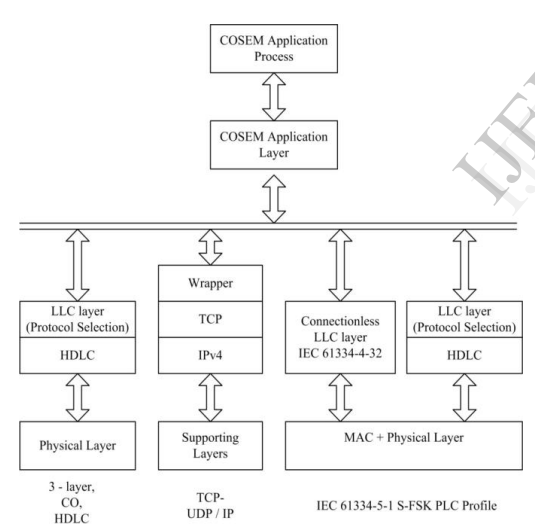
\includegraphics[width=0.7\textwidth]{gfx/Dlms_osi.png}
   \caption{
       DLMS/COSEM Kommunikationslayer
   }
   \source{\cite{vyas2012advance}}
   \label{fig:dlmsOsi}
\end{figure}

Der Applicationlayer des \ac{DLMS} Protokolls definiert die Funktionen eines intelligenten Stromzählers als Objekte \parencite{vyas2012advance}.

\subsection{COSEM}\label{cosem}
Der \ac{COSEM} Standard, welcher teil von \ac{DLMS} ist, beschreibt eine Sammlung von logischen Geräten, welche gemeinsam in einem physischen Gerät untergebracht werden.
Diese logischen Geräte bestehen aus mehreren Attributen und Methoden, welche jeweils zu Objekten zusammengefasst sind.
Spezifische Objekte können mittels \ac{OBIS} Code adressiert werden.
Die Schnittstellen zu den Objekten sowie eine Liste von standard \ac{OBIS} Codes sind in \ac{COSEM} enthalten  \parencite{vyas2012advance}.


\section{Landis+Gyr intern}\label{lgintern}
In den folgenden Abschnitten werden Konzepte, Anwendungen und Produkte erklärt, welche bei der Landis+Gyr intern verwendet werden.

\subsection{Picasso Platform}\label{picasso}
Picasso ist der Name einer Software Platform der Landis+Gyr.
Mehrere Teams, verteilt auf vier Kontinente, arbeiten am C++ Code dieser Platform.
Sie beinhaltet grundlegende Komponenten wie beispielsweise das Betriebs- und Filesystem sowie Funktionen welche von allen Produkttypen verwendet werden.
Die Teams welche die konkreten Stromzähler-Produkte entwickeln, bauen auf Picasso auf und ergänzen die Platform um Funktionen, welche nur von ihrem Produkt verwendet werden.
Damit die Platform mit unterschiedlichen Konfigurationen getestet werden kann, verfügt sie über mehrere Referenzprodukte.
Referenzprodukte sind Produkte, welche nicht Verkauft werden, sondern nur für interne Zwecke verwendet werden.
Am Standort Cham arbeitet ein Team an der Platform sowie eines an einem Produkt, dem Stromzähler Model \textit{E660}.
Der Autor dieser Arbeit ist seit mehreren Jahren Teil des Platformteams.



\subsection{Object Model und Class Description}\label{objectModelsClassDescriptions}
Im Absatz \ref{cosem} wurde erwähnt, dass die Funktionen eines intelligenten Stromzählers mittels Objekten abstrahiert werden.
Bei der Landis+Gyr werden alle Objekte eines bestimmten Produkts jeweils in einem Object Model zusammengefasst.
Anhand des Object Models entwerfen Architekten die Funktionen eines Zählers.
Sie verwenden eine Excel Tabellen um die Werte der Object Models zu bearbeiten.
In Abbildung \ref{fig:objectModel} ein der Header sowie ein Objekt aus einer solchen Tabelle dargestellt.

\begin{figure}[H]
   \centering
   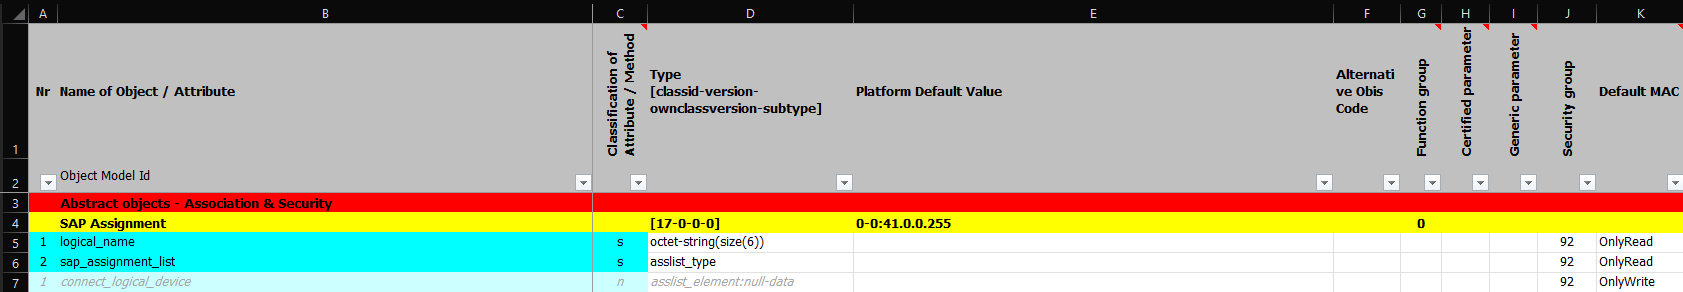
\includegraphics[width=1.0\textwidth]{gfx/objectModel.png}
   \caption{
       Ausschnitt aus der Excel Tabelle eines Object Models
   }
   \label{fig:objectModel}
\end{figure}

Diese Objekte sind jeweils Instanzen von \ac{COSEM} Klassen.
Die Funktionalität und Schnittstelle dieser Klassen sind in sogenannten Class Descriptions dokumentiert.
Jede Class Description ist in einem eigenen Word Dokument abgelegt.
Ein Beispiel dazu in in Abbildung \ref{fig:classDescription} ersichtlich.

\begin{figure}[H]
   \centering
   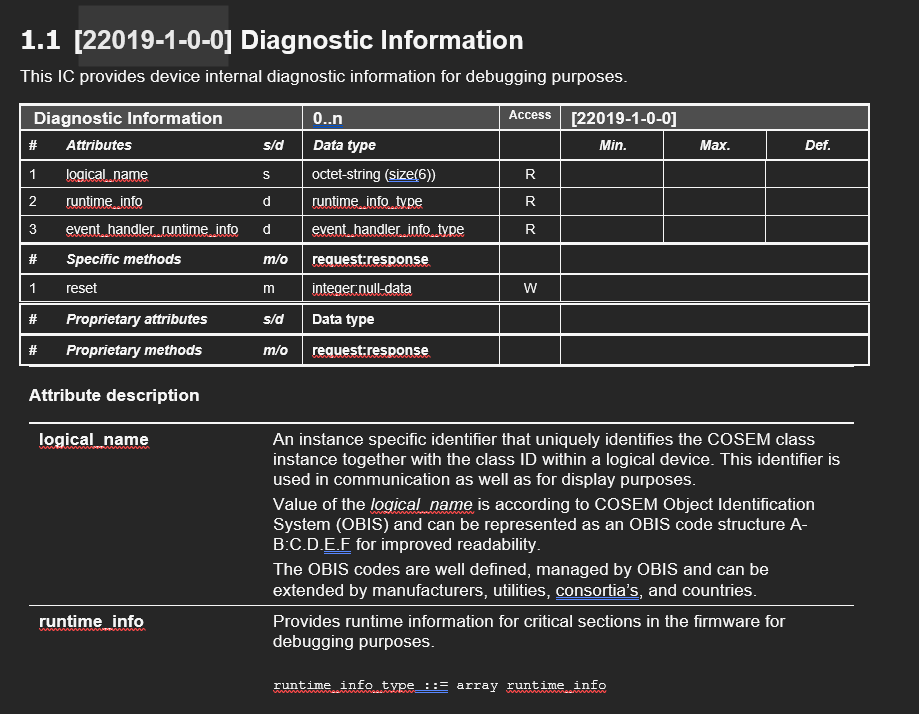
\includegraphics[width=1.0\textwidth]{gfx/ClassDescription.png}
   \caption{
       Ausschnitt aus einer Class Description
   }
   \label{fig:classDescription}
\end{figure}

Das Object Model in Kombination mit den verwendeten Class Descriptions dient bei der Firmwareentwicklung als Referenz für die Implementation der \ac{DLMS}/\ac{COSEM} Schnittstelle.
Um die Integrität dieser Dateien sicherzustellen und um diese in andere Dateiformate zu konvertieren, entwickelt und betreibt die Landis+Gyr mehrere Programme.
Diese werden im nächsten Abschnitt erläutert.

\subsubsection{Tools}
Das Programm \textit{Picasso Tools} stellt ein Plugin für Excel bereit, welches dem Benutzer ermöglicht den Inhalt eines Object Models zu validieren.
Dabei werden die Objekte anhand von vordefinierten Regeln auf Korrektheit und Vollständigkeit überprüft.
Des Weiteren wird mithilfe der entsprechenden Class Description überprüft, ob die Attribute und Methoden eines Objekts korrekt sind.
Die Class Descriptions müssen dazu als XML Dateien vorhanden sein.
Da die Class Descriptions wie zuvor beschrieben jedoch Word Dokumente sind, müssen diese mit dem Programm \textit{Description Tools} exportiert werden.
Analog zu \textit{Picasso Tools} stellt \textit{Description Tools} ein Plugin, in diesem Fall für Word, bereit, welches Dokumente validieren und als XML exportieren kann.

Nebst den Plugins bieten beide Programme auch ein \ac{CLI} an.
Dieses wird von einem Server verwendet, welcher jeden Tag alle Object Models und Class Description validiert und als XML exportiert.
Anhand der Validierungsresultate erstellt er einen Report, welche einen Überblick über die Qualität der Dokumente gibt sowie auf Fehler hinweist.

Beide Tools sind in der Programmiersprache C\# entwickelt und nutzen die Komponente \textit{InfraLib}.
Diese ist eine C\# Bibliothek, welche Funktionalitäten wie das Parsen der XML files anbietet. 
\footnote{\textit{Picasso Tools}, \textit{Description Tools} sowie \textit{InfraLib} wurden vom Autor dieser Arbeit erstellt, als dieser seine Berufslehre bei der Landis+Gyr absolvierte und seither weiterentwickelt }

\subsection{Firmwareentwicklung}\label{fwEntwicklung}
Am Standort Cham entwickelt die Landis+Gyr Firmware für intelligent Stromzähler.
Dazu wird die Programmiersprache C++ eingesetzt.
Wie im Abschnitt \ref{objectModelsClassDescriptions} bereits erwähnt, stützt sich die Firmware auf Object Models.
Diese werden verwendet, um jenen Code zu generieren, welcher die \ac{COSEM} Objekte in der Firmware instanziert.
Ein Tool, welches in der Programmiersprache Python geschrieben ist, parst die XML Repräsentation des Object Models und mit Hilfe von Templates den entsprechenden Code.
Da das verwendete Buildsystem, SCons \footnote{https://scons.org/}, ebenfalls mit Python arbeitet ist Python hinter C++ die zweit meist verwendete Sprache im Projekt der Firmwareentwicklung.

\subsection{E66C Testing}\label{pythonTesting}
\textit{E66C} ist die Modellbezeichnung eines Kommunikationsmoduls, welches von der Landis+Gyr in Cham entwickelt wird.
Dabei handelt es sich um eine Komponente, welcher auf gewisse Stromzählermodelle aufgesteck werden kann und diesen um Kommunikationsfunktionen erweitert.

\begin{figure}[H]
   \centering
   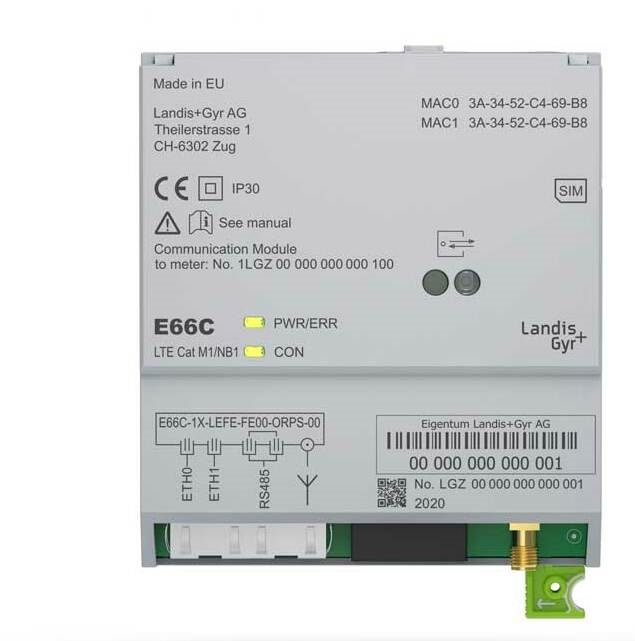
\includegraphics[width=0.7\textwidth]{gfx/landis-e66c.jpg}
   \caption{
      Kommunikationsmodule E66C der Landis+Gyr
   }
   \source{Landis+Gyr AG}
   \label{fig:e66c}
\end{figure}

Um das Zusammenspiel des \textit{E66C} mit einem Stromzähler automatisiert zu testen, entwickelte das Team in Cham das Programm \textit{libpydlms}.
Dieses ermöglicht das Lesen und Schrieben von \ac{COSEM} Objekten in der Sprache Python.


\subsection{ATS}\label{ats}
\ac{ATS} ist eine Software welche für das Testen von intelligenten Stromzählern verwendet wird.
Dazu werden Testscripts in einer \ac{ATS} spezifischen Scriptsprache benötigt.
Über diese Scripts könne Werte des Zählers über die \ac{DLMS} Schnittstelle geschrieben, ausgelesen und mit Erwartungswerten vergleichen werden.
Zusätzlich ist die Steuerung der Testumgebung möglich.
Befindet sich der Testaufbau beispielsweise auf dem Tisch des Entwicklers, so wird der Stromzähler in der Regel nicht über eine richtige Stromquelle betrieben sondern an einen Emulator angeschlossen, welcher diese ersetzt.
In diesem Fall wird der Emulator über das \ac{ATS} Testscript gesteuert.

Die \ac{ATS} wurde von der Landis+Gyr in der Programmiersprache C\# entwickelt und wird aktuell für das Testen aller Stromzähler der Picasso Platform (siehe \ref{picasso}) eingesetzt.



\subsection{DMT2}\label{dmt}
Die Software \ac{DMT2} wurde für die Landis+Gyr von einem externen Lieferanten entwickelt.
Mit ihr können Scripts geschrieben und ausgeführt werden, welche mittels \ac{DLMS} mit intelligenten Stromzähler kommunizieren.
Diese Scripts können um einfach Benutzeroberflächen erweitert werden, welche mit XML deklarativ definiert werden.
Verwendet werden diese, um Interaktionen, welche die Entwickler oft durchführen müssen, zu vereinfachen.
In Abbildung \ref{fig:dmt2logger} wir beispielsweise ein Script und die dazugehörige Benutzerschnittstelle für die Laufzeitkonfiguration des Loggers eines Zählers gezeigt.
Wenn dort beispielsweise das Log Level verändert wird, schreibt das Script den entsprechenden Wert automatisch in die korrekte \ac{COSEM} Klasse.
\begin{figure}[H]
   \centering
   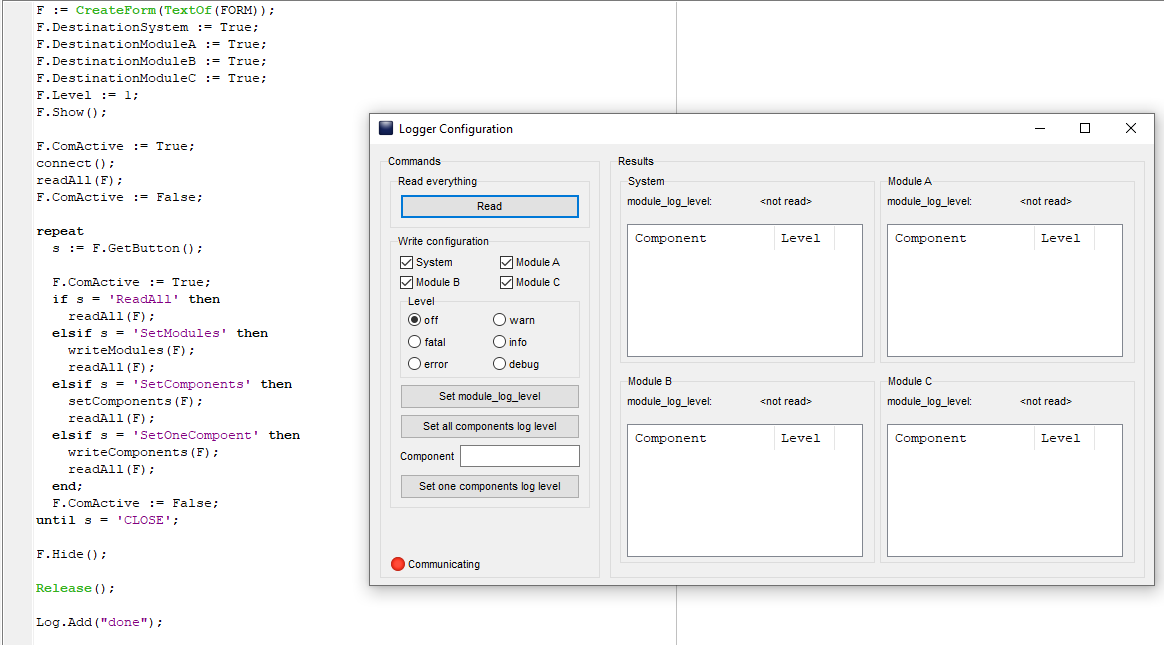
\includegraphics[width=1.0\textwidth]{gfx/dmt2logger.png}
   \caption{
      Ausschnitt aus \ac{DMT2} mit geladenem Logger-Konfigurationsscript
   }
   \label{fig:dmt2logger}
\end{figure}

Eine weitere Funktion des \ac{DMT2} ist \textit{Quick Access}.
Diese ermöglicht das Lesen und Schrieben einzelne Attribute sowie das ausführen von Methoden.
Das Ziel dieser Arbeit ist es, die Funktionalität des \textit{Quick Access} durch eine neue Softwarelösung zu ersetzten.
Im folgenden Abschnitt werden einige Stärken und Schwächen des \ac{DMT2} aufgezeigt.
Diese basieren auf einer Umfrage, welche unter den Benutzern des \ac{DMT2} durchgeführt wurde.
Im Abschnitt \ref{survey} ist mehr zur Umfrage zu lesen.

\subsubsection{Stärken}
\begin{itemize}
   \item Die Anwendung läuft stabil, Abstürze kommen sehr selten vor.
   \item Es kann zwischen verschiedenen Kommunikationseinstellungen gewechselt werden. Dazu muss jeweils eine entsprechende Datei geladen werden.
\end{itemize}

\subsubsection{Schwächen}
\begin{itemize}
   \item Fehlermeldungen werden als Dialog angezeigt und müssen jeweils bestätigt werden um fortzufahren.
   \item Es ist schwierig, nach spezifischen Objekten zu suchen.
   \item Das ausführen von Methoden und Schrieben von Attributen ist umständlich. Die Parameter müssen in einer XML Struktur eingetragen werden, welche anfällig für Fehler ist.
   \item Es wird jeweils nur die Antwort des zuletzt ausgeführten Befehls angezeigt.
   \item Es ist Umständlich mehrere Instanzen des \ac{DMT2} gleichzeitig zu nutzen. 
\end{itemize}


\section{WinUI3}
WinUI3 ist eine Platform, welche es erlaubt native Benutzeroberflächen für Windows zu entwickeln.
Sie ist teil der Windows APP SDK \footnote{https://docs.microsoft.com/en-us/windows/apps/windows-app-sdk/}.
Der Quellcode dazu ist Open Source \parencite{winuiintro}.
WinUI3 wird Microsoft als beste Technologie zur Erstellung von Benutzerschnittstellen bezeichnet und löst ältere Technologien wie \ac{WPF} oder \ac{UWP} ab.
Die erste stabile Version ist seit November 2021 verfügbar.
Neue Updates sollen regelmässig veröffentlich werden.
WinUI3 kann in Kombination mit dem .Net Framework von Microsoft verwendet werden, ist jedoch nicht davon abhängig.
Es werden die Programmiersprachen C\# und C++ unterstützt \parencite{winuiroadmap}.


% https://dvmarcilio.github.io/papers/icpc2019.pdf
% http://aagasc.edu.in/cs/books/Software%20Quality%20Assurance%20From%20Theory%20to%20Implementation.pdf
% see document in Downloads!

\section{Softwarequalität}\label{softwarequality}
In der DIN-ISO-Norm 9126 wird Software Qualität so definiert:
\dq Software-Qualität ist die Gesamtheit der Merkmale und Merkmalswerte eines Software-Produkts, die sich auf dessen Eignung beziehen, festgelegte Erfordernisse zu erfüllen.\dq

\citeauthor{hoffmann2013software} (\citeyear{hoffmann2013software}) hebt zu dieser Definition hevor, dass es nicht ein einziges Kriterium gibt, welches die Qualität von Software misst.
Vielmehr ist es eine Kombination verschiedener Kriterien.
Auf diese wird im folgenden Abschnitt (\ref{kriterien}) eingegangen.
Die Software-Qualitätssicherung befasst sich mit Methoden welche eingesetzt werden können, um bei diesen Kriterien gut abzuscheiden.
Sie wird in im Abschnitt \ref{qualisicherung} behandelt.

\subsection{Kriterien}\label{kriterien}
In den folgenden Abschnitten werden die Kriterien erklärt, welche nach \citeauthor{hoffmann2013software} relevant sind für die Softwarequalität.
Die ersten vier Kriterien sind dabei für den Kunden wichtig, da diese direkte Auswirkung auf ihn haben.
Die letzteren vier sind nur für den Hersteller der Software relevant.
\subsubsection{Funktionalität}
Die Funktionalität gibt an, ob die spezifizierten Anforderungen erfüllt sind.
Funktionale Fehler werden meist durch Bugs in der Implementierung verursacht, können ihren Ursprung jedoch auch in fehlenden oder falsche verstandenen Spezifikationen haben.
Sie können durch den Einsatz von Software-Qualitätsicherungstools vorgebeugt werden.

\subsubsection{Performance}
Mit Performance sind die Anforderungen an die Software während deren Laufzeit gemeint.
Für einfache Desktop Anwendungen stellt dieses Kriterium meist kein Problem dar.
Handelt es sich bei der Anwendungen jedoch um ein Echtzeitsystem, so ist die Performance eines der wichtigsten Kriterien.

\subsubsection{Zuverlässigkeit}
Mit diesem Kriterium ist gemeint, wie zuverlässig eine Software ihre Funktionen ausführt.
Kommt es oft zu Fehlern oder Abstürzen, so ist die Zuverlässigkeit tief.
Sie ist stark an die anderen Kriterien gekoppelt.
Hat die Software inkorrekte Funktionalität oder schlechte Performance, so ist auch die Zuverlässigkeit tief.

\subsubsection{Benutzbarkeit}
Die Eingenschaften einer Software, welche mit dem Menschen interagieren, sind in diesem Kriterium zusammengefasst.
Im Abschnitt \ref{usability} wird diese Thematik vertieft.

\subsubsection{Wartbarkeit}
Um eine Software auch nach der ersten Inbetriebnahme weiter zu entwickeln, so muss diese Wartbar sein.
Es soll möglich sein, erkannte Bugs einfach zu beheben.
Die Software soll so aufgebaut sein, dass sie nicht vollständig umgebaut werden muss, nur um eine neue Funktion hinzuzufügen.


\subsubsection{Transparenz}
Mit diesem Kriterium wird bewertet, wie transparent das Program intern umgesetzt ist.
Alle Teilkomponenten der Software sollen einfach zu verstehen sein.
Tendenziell verschlechtert sich die Transparenz im verlaufe der Weiterentwicklungen.


\subsubsection{Übertragbarkeit}
Die Übertragbarkeit gibt an, ob sich eine bestehende Software in eine andere Umgebung übertragen lässt.
Kann ein Programm nur auf einer bestimmten Betriebssystemversion oder gar nur auf einem einzigen Rechner ausgeführt werden, so ist dessen Übertragbarkeit sehr schlecht.
Mit Umgebung ist jedoch nicht nur die technische Umgebung wie das Betriebssystem gemeint sonder sie kann auch Aspekte wie die Sprache oder Kultur beinhalten.

\subsubsection{Testbarkeit}
Software ist meist so komplex, dass es nicht ausreicht lediglich die Benutzerschnittstellen zu testen.
Die möglichen Kombinationen von Eingabeparametern sind dabei viel zu umfangreich.
So müssen einzelne Komponenten einzeln getestet werden.
Dies ist nur möglich, wenn diese so entwickelt werden, dass sie auch testbar sind.
Damit ist gemeint, dass bspw. ein Algorithmus so implementiert ist, dass er von keinerlei internen Zustände der Anwendungen abhängig ist. 


\subsection{Software-Qualitätssicherung}\label{qualisicherung}
Unter Software-Qualitätssicherung versteht sich eine systematische und geplante Sammlung von Aktionen, 
welche die Sicherheit geben, dass die erstellte Software den Anforderungen entspricht.
Diese sollen den Entwicklungsprozess evaluieren und sicherstellen,
dass die Software im gegebenen zeitlichen sowie finanziellen Rahmen erstellt werden kann \parencite{galin2004software}. 

Sie unterscheidet sich von der Qualitätskontrolle indem sie nicht das fertige Produkt sondern den Herstellungsprozess evaluiert und prüft \parencite{galin2004software}.
Die beiden Teile, Produktqualität und Prozessqualität, aus welchen sich die Software-Qualitätssicherung nach \citeauthor{hoffmann2013software} zusammensetzt, werden in den nächsten Abschnitten erläutert.

\subsection{Produktqualität}
Zur Sicherung der Produktqualität gehören jene Ansätze welche einen direkten Einfluss auf das Produkt und somit auf die zuvor genannten Kriterien haben.
In nächsten Abschnitten werden einige Techniken und Methoden erklärt, welche laut \citeauthor{hoffmann2013software} bei der Sicherung der Produktqualität helfen.

\subsubsection{Software-Richtlinien}
Software-Richtlinien sind Konventionen, welche vorgehen, wie mit einer bestimmten Programmiersprache gearbeitet werden soll.
Sie befassen sich dabei mit jenem Teil, welcher von der Syntaktik und Semantik einer Sprache nicht vorgegeben ist.
Ihr Ziel ist es, die geschriebene Software zu vereinheitlichen.
Dies verhindert, dass die Teile einer Software in unterschiedlichen Programmierstielen geschrieben sind, in welche sich jeweils mit viel Zeitaufwand eingearbeitet werden muss.
Des Weiteren sollen sie zu Fehlerreduktion führen, indem einheitliche Lösungsmuster vorgeschrieben werden sowie fehleranfällige Sprachkonstrukte verboten werden.

Die folgenden Punkte sind Beispiele, welche in einer typischen Richtlinie vorhanden sein können:
\begin{itemize}
   \item Die Schreibweise von Bezeichnern (z.B. Pascal Case)
   \item Die Verwendung von Einrückungen, Leerzeichen und Zeilenschaltungen
   \item Vorgaben, welche Codeteile wie Dokumentiert werden
\end{itemize}
Einige Konventionen, wie beispielsweise die \textit{MISCRA-C}\footnote{https://www.misra.org.uk/} Sprachkonvention, geben des Weiteren konkrete Vorgaben zur Verwendung bestimmter Sprachkonstrukte an.
In Abbildung \ref{fig:misra} ist ein Ausschnitt aus \textit{MISCRA-C} abgebildet.
\begin{figure}[H]
   \centering
   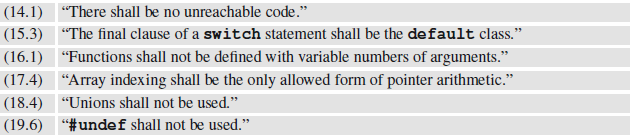
\includegraphics[width=1.0\textwidth]{gfx/misra.png}
   \caption{
      Ausschnitt aus der \textit{MISCRA-C} Sprachkonvention
   }
   \source{\cite{hoffmann2013software}}
   \label{fig:misra}
\end{figure}


\subsubsection{Typisierung}
Die Verwendung eines Typisierungssystem steigert die Qualität einer Software.
Mittels statischer Typprüfung wird durch den Compiler geprüft, ob die verwendete Typen jeweils korrekt sind.
Die dynamische Typprüfung, welche meist von einem Interpreter durchgeführt wird, erkennt falsch verwendete Typen bei Laufzeit und kann so Programmabstürze verhindern.

Viele Programmiersprachen bieten eine statische oder dynamische Typprüfung an.
Einige, wie bspw. C\# sogar beide.

\subsubsection{Portabilität}
Bei der Portabilität geht es nicht direkt darum, dass eine Software auf allen erdenklichen Systemen läuft, sondern vielmehr, dass die Portierung auf ein neues System mit geringem Aufwand vollbracht werden kan.
Dazu gehört, dass nur jene Codeteile angepasst oder neu geschrieben werden müssen, welche effektiv eine Abhängigkeit zum jeweiligen System haben.
Die Businesslogik einer Anwendung ist typischerweise eher unabhängig von einem System, währen die Benutzerschnittstelle stark an ein bestimmtes Betriebssystem gekoppelt sein kann.
Um die Portabilität zu gewährleisten, soll der Code von Anfang an so organisiert werden, dass plattformunabhängige Komponenten sauber von den plattformabhängigen getrennt sind.

\subsubsection{Fehlertolerante Programmierung}
Software-Systeme reagieren unterschiedlich auf Fehler.
Bei Desktop Anwendungen im Büroumfeld ist der Absturz einer Anwendung nicht vorteilhaft, wird jedoch von Nutzern akzeptiert.
Bei sicherheitskritischen Systemen ist dies nicht der Fall.
Software, welche bswp. die Unversehrtheit von Personen tangieren, muss so programmiert werden, dass sie mit Fehlern umgehen kann.
Ein Ansatz dazu ist, das Teile des Systems mehrfach vorhanden sind.
Diese Redundanz führt dazu, das ein Ausfall eines Teiles nicht zum Absturz des ganzen Systems führt.

Bei jeder Art von Software ist die Ausnahmebehandlung da, um mit spontan aufgetretenen Fehlern umzugehen.
Geplante Ausnahmen, wie beispielsweise ungültige Eingaben eines Nutzers können Behandelt werden und dem Benutzer entsprechend mitgeteilt werden.
Ungeplanten Ausnahmen, wie beispielsweise eine Division durch Null, können behandelt werden, um einen Absturz des Programms zu verhindern.


\subsubsection{Software-Test}
Bei Software-Tests wird eine Komponente mit vordefinierten Eingabewerten und bestimmten Zuständen ausgeführt.
Das Ergebnis wird mit einem Erwartungswert abgeglichen.
So kann sichergestellt werden, dass eine Komponente so funktioniert wie sie soll.
Da Tests nicht nur auf der Ebene einer einzelnen Komponente geschrieben und ausgeführt werden können sondern auch das Zusammenspiel mehrere Komponente oder ganzer System testen können,
sind sie für das Kriterium der Funktionalität sehr wichtig.
Sie sind somit ein wichtiger Bestandteil eines Softwareprojekts.
%todo evtl schrieben, dass tests selbst hohe quali haben müssen
Während des Schreiben von Tests zeigt sich auch, zu welchem Grad das Kriterium der Testbarkeit erfüllt ist.

Testmetriken geben Auskunft zu einer Testmenge.
Sie geben an, ob eine Komponente ausreichen getestet wurde und welche Teile des Codes noch nicht getestet sind.

\subsubsection{Statische Analyse}
Im Gegensatz zu den im vorherigen Abschnitt erwähnten Software-Tests wird bei der statischen Analyse der zu bewertenden Code nicht ausgeführt.
Vielmehr werden Aspekte des Codes systematisch quantitativ erfasst.
Dies wird automatisiert mit einer entsprechenden Software gemacht und kann folgende Punkte beinhalten:
\begin{itemize}
   \item Metriken, welche die Software in Punkten wie beispielsweise Komplexität, Wartbarkeit oder Kohäsion beurteilen.
   \item Überprüfung, ob Software-Richtlinien eingehalten wurden.
   \item Erkennen von Anomalien oder Sicherheitslücken im Code.
\end{itemize}

Im Abschnitt \ref{quality:sonar} wird das Programm SonarQube vorgestellt, welches für solche statischen Analysen eingesetzt werden kann.

\subsection{Prozessqualität}
Die in den folgenden Abschnitte erklärten Massnahmen zur Verbesserung der Prozessqualität haben keine direkten Einfluss auf die Qualitätskriterien.
Vielmehr bilden sie eine Grundlage um überhaupt qualitative Software erstellen zu können.

\subsubsection{Build- \& Test-Automatisierung}
Bei der Build- \& Test-Automatisierung geht des darum, dass das Kompilieren der Software sowie das Ausführen von Software-Tests ohne manuellen Aufwand auf einem Server ausgeführt wird.
Dies kann beispielsweise bei jedem Commit oder jeder neuen Version der Software geschehen.
Das Ziel dabei ist, dass neue Defekte möglichst rasch erkannt werden.
Werden die Testresultate über einen längeren Zeitraum abgelegt, so lassen dieses Rückschlüsse auf die Stabilität einzelner Softwarekomponenten zu.

\subsubsection{Vorgehensmodelle}
Als Vorgehensmodell soll eine bewährte Methodik gewählt werden, welche vorgibt, wie das Softwareprojekt konkret umgesetzt wird.


\subsubsection{Versionsverwaltung}
Ein Versionsverwaltungsystem ist ein Repository, welches alle Artefakte die zur Erstellung der Software benötigt werden speichert und bei Änderungen deren Versionen verwaltet.
Bei einem solchen System sind unter anderem folgenden Punkte wichtig:
\begin{itemize}
   \item Die gemachten Änderungen sollen transparent protokolliert sein.
   \item Es soll möglich sein, jederzeit auf ältere Versionen des Codes zuzugreifen.
   \item Entwickler müssen gleichzeitig am selben Code arbeiten können
\end{itemize}



\subsection{SonarQube}\label{quality:sonar}
SonarQube ist eine Software-Qualitatssicherungstool, welches Code analysiert und Berichte zur Codequalität erstellt.
Die Berichte könne beispielsweise Code-Style-Verletzungen, Designfehler oder gar Sicherheitslücken aufzeigen.
Da die Analysen statisch sowie dynamisch durchgeführt werden, können auch Metriken zu Codeabdeckung durch Tests erstellt werden \parencite{malloy_2021}.
SonarQube berichtet nicht nur über erkannte Probleme sondern beinhaltete auch Funktionen um diese zu Verwalten.
Ein Problem kann beispielsweise direkt der Person zugewiesen werden, welche es bearbeiten soll.
Meldungen, welche nicht bearbeitet werden, können entsprechend markiert werden, so dass sie in Zukunft nicht erneut auftreten.
Da SonarQube die Historie der Berichte speichert, werden neue Probleme speziell hervorgehoben.
Wie sich die totale Anzahl der Problem über die Zeit entwickelt, wird ebenfalls angezeigt und gibt einen Trend der Softwarequalität an.

% Maintainability, Security, Reliability, Complexity

\subsubsection{Funktionsweise}\label{sonar:funktionsweise}
In einem produktiven Umfeld ist die Funktionsweise von SonarQube wie folgt:
SonarQube wird auf einem Server installiert und mit einem \ac{CI} Server verbunden.
Wenn Entwickler Änderungen am Code in das jeweilige \ac{SCM} System pushen löst dies einen Build auf dem \ac{CI} Server aus.
Dieser Build beinhaltet Sonar Scanner.
Ist der Build abgeschlossen werden die Berichte der Scanner an die SonarQube Instanz übermittelt.
Dort werden sie verarbeitet, in der Datenbank abgelegt und über eine Benutzerschnittstelle dargestellt \parencite{malloy_2021}.

\subsection{Qualitätssicherungstools bei der Landis+Gyr}
Für die Qualitätssicherung der Firmware setzt die Landis+Gyr aktuell C-STAT\footnote{https://www.iar.com/cstat} für statische Codeanalysen ein.
Eine kürzlich durchgeführte Evaluation hat jedoch ergeben, dass SonarQube die geeignetere Lösung wäre.
Dieser Umstieg ist zum Zeitpunkt dieser Arbeit bereits geplant, jedoch noch nicht realisiert.
Bei den verschiedenen C\# Projekten, welche in diesem Kapitel genannt wurden, werden keinerlei Qualitätsicherungstools eingesetzt.

\section{Usability}\label{usability}
Ins Deutsche übersetzt bedeutet Usability nach \citeauthor{usability} (\citeyear{usability}) Gebrauchstauglichkeit oder Nutzerfreundlichkeit.
Sie sorgt dafür, dass Programme einfach verwendet werden können.
Gemessen wird sie daran, wie schnell und direkt ein Benutzer sein Ziel während der Nutzung der Software erreicht.
Die Norm DIN EN ISO 9241 beschreibt einige Eigenschaften, welche eine Anwendung mit hoher Usability haben soll.
Diese sind:
\begin{itemize}
   \item der Aufgabe angemessen
   \item selbst beschreibend
   \item steuerbar
   \item erwartungskonform
   \item fehlertolerant
   \item lernförderlich
   \item motivierend
\end{itemize}
Um diese Eigenschaften zu erreichen, ist ein entsprechendes Vorgehen während der Entwicklung nötig.
Dies wir im nächsten Abschnitt erläutert.


\subsection{Projektablauf mit Usability als Ziel}
\citeauthor{usability} (\citeyear{usability}) sagen, dass die Nutzer während der Entwicklung möglichst früh eingebunden werden.
So kann von ihnen die Bestätigung eingeholt werden, dass das Entwickelte gefällt.
Wenn es nicht gefällt, so kann wieder von vorne angefangen werden.
Laut \citeauthor{usability} ist in einem optimalen Projektablauf der Nutzer in jeder Phase eingebunden.
So soll in einer ersten Phase der Nutzer kennengelernt und verstanden werden.
Dazu werden im folgenden Abschnitt einige Methoden erklärt.
In einer nächsten Phase sollen die Anforderungen der Nutzer spezifiziert werden.
Diese sollen in der dritten Phase anhand von Prototypen umgesetzt und in der letzten Phase von den Nutzern evaluiert werden.
Agile Vorgehensmodelle eignen sich gut, um regelmässig Tests mit den Nutzern durchzuführen, beispielsweise nach jedem Sprint.
Die vier erwähnten Phase können wiederholt durchgeführt werden.
Um in der vierten Phase möglichst positive Testergebnisse zu erhalten, gibt es Richtlinien, welche befolgt werden können.
Auf diese wird in Abschnitt \ref{guidelines} genauer eingegangen.


\subsection{Methoden um die Nutzer kennen zu lernen}
Um Anforderungen an die Anwendung formulieren zu können, sollen zuerst die Nutzer dieser Anwendung kennengelernt und deren Bedürfnisse sowie Wünsche erfasst werden.
\citeauthor{usability} (\citeyear{usability}) nennen dazu mehrere Methoden.
Diese werden hier vorgestellt:

\subsubsection{Fokusgruppen}\label{fokusgruppe}
Bei einer Fokusgruppe handelt es sich um eine Gruppendiskussion.
Ein Moderator führt mit fünf bis zehn Personen ein Gespräche zu einem bestimmten Thema.
So können bestehende Anwendungen verbessert oder Ideen für neue gesammelt werden.
Ein erstelltes Konzept kann den Nutzern erstmals gezeigt und von ihnen evaluiert werden.
Der Austausch innerhalb der Fokusgruppe soll gefördert werden, da dies die Kreativität anregt.
Es kann hilfreich sein, wenn sich die Teilnehmer der Diskussion im Voraus auf diese vorbereiten.
So sind sie gezwungen, bereits vor der Diskussion eine Meinung zu bilden und es kann vermieden werden, dass sich Teilnehmer der Gruppenmeinung anschliessen.


\subsubsection{Befragungen}\label{befragung}
Ziel einer Befragung ist es, die individuellen Meinungen von Einzelpersonen zu erfassen.
In der Regel werden sie mithilfe eines Fragebogens durchgeführt.
Im Gegensatz zu den Fokusgruppen sind sie eher dazu da, um quantitative Daten zu erheben und weniger für die Erfassung neuer Ideen geeignet.
Wird dieselbe Befragung über längere Zeit mehrmals durchgeführt, können Veränderungen oder Trends gemessen werden.


\subsubsection{Vor-Ort-Beobachtungen}\label{vorort}
Bei einer Vor-Ort-Beobachtung wird der Benutzer aus dem Hintergrund bei einer typischen Nutzungssituation beobachtet.
Er soll dabei vom Beobachter möglichst wenig beeinflusst werden, so dass seine Abläufe möglichst alltäglich sind.
Der Beobachter notiert, wie die Software verwendet wird.
Dabei soll speziell auf unbewusstes Verhalten der Nutzer geachtet werden.


\subsubsection{Tagebuchstudien}\label{tagebuchstudien}
Bei Tagebuchstudien erfassen die Nutzer ihr eigenes Verhalten.
Entweder bei der Nutzung einer konkreten Anwendung oder in Situationen bei denen eine geplante Anwendung eingesetzt werden soll.
So können Erlebnisse der Nutzer über einen längeren Zeitraum gesammelt werden.
Ereignisse und Erfahrungen welche unregelmässig oder gar einmalig auftreten, können so erfasst werden.
Dies ist bei Vor-Ort-Beobachtungen nur schwer möglich.

\subsection{Usability Guidelines}\label{guidelines}
Bewährte Guidelines können befolgt werden, um eine hohe Usability zu erreichen.
\citeauthor{usability} (\citeyear{usability}) kennen Guidelines zu unterschiedlichen Aspekten einer Anwendungen.
Einige dieser Aspekte und die zugehörigen Guidelines werden in den folgenden Abschnitten erläutert.

\subsubsection{Informations- und Navigationsarchitektur}
Die Informations- und Navigationsarchitektur bildet das Fundament einer Anwendung.
Während sie bei kleineren Anwendungen noch vernachlässigt werden kann, so muss sie bei grösseren Anwendungen ausführlich geplant werden.
Das Ziel einer guten Informations- und Navigationsarchitektur ist, dass ein Nutzer schnell und einfach zu den gewünschten Informationen navigieren kann.
Dies kann erreicht werden, indem die Inhalte zuerst grob sortiert werden.
Diese Sortierung wird dann als Grundlage genommen, um eine feine Gliederung zu erarbeiten.
Dabei ist wichtig, dass nicht ein perfektes, logisches System das Ziel ist, sondern eine Architektur, welche für den Nutzer intuitiv zu bedienen ist.


\subsubsection{Gestaltungsraster}
Gestaltungsraster sind dazu da, um die Elemente einer Benutzeroberfläche geordnet darzustellen.
Im Gestaltungsraster wird die Seite oder das Fenster mittels Führungslinien in Reihen und Spalten eingeteilt.
Diese Linien geben an, wo Elemente platziert werden können und wie viel Abstand zwischen ihnen ist.
In Abbildung \ref{fig:Gestaltungsraster} sind mehrere solcher Raster aufgezeigt.
\begin{figure}[H]
   \centering
   
\includegraphics[width=1.0\textwidth]{gfx/Gestaltungsraster_aus_buch.png}
   \caption{
      Verschiedene Gestaltungsraster welche mittels Führungslinien unterteilt sind.
   }
   \source{\citeauthor{usability}}
   \label{fig:Gestaltungsraster}
\end{figure}
Bereits die ersten Entwürfe der Benutzerschnittstelle sollen auf ein Raster gezeichnet werden.
Bei der Programmierung der Benutzerschnittstelle können diese Einteilungen direkt übernommen werden.


\subsubsection{Farben}
Farben sind für die Gestaltung von Benutzerschnittstellen sehr wichtig.
Ansprechende Anwendungen machen bei der Nutzung Freude und hinterlassen einen positiven Eindruck.
Die Auswahl von Farben und was als ästhetisch wahrgenommen wird, ist subjektiv.
Trotzdem gibt es einige Richtlinien, welche befolgt werden können:
\begin{itemize}
   \item Bestimmte Farben werden oft der gleichen Eigenschaft zugeordnet. So bedeutet Grün of \dq In Ordnung\dq, während Rot oft mit \dq Gefahr\dq in Verbindung gebracht wird. Solche Eigenschaften sollen gezielt eingesetzt werden.
   \item Wichtige Elemente einer Anwendungen können mit auffälligen Farben hervorgehen werden.
   \item Bei Anwendungen, welche über längere Zeit verwendet werden, sollen Farben sparsam eingesetzt werden, da diese Ablenken können.
   \item Der Kontrast zwischen Vorder- und Hintergrund soll gross genug sein, damit beispielsweise Text auch bei erschwerten Bedingungen wie Sonnenschein gelesen werden kann.
   \item Um zwei unterschiedliche Elemente zu unterscheiden, sollte nicht einzig auf unterschiedliche Farben gesetzt werden. Menschen tun sich schwer damit, Farben zu unterscheiden.
Für Personen mit einer Rot-Grün-Schwäche ist es teilweise gar unmöglich.
\end{itemize}


\subsubsection{Icons}
Icons bieten die Möglichkeit, platzsparend Auskunft über die Funktion eines Elements wie z.B. einem Knopf zu geben.
Ästhetisch bieten Icons eine ansprechende Abwechslung zu Text.
Gängige Icons wurden von den Benutzern bereits gelernt und kommen ihnen vertraut vor.
Trotzdem sollten Icons wenn möglich mit einem Label beschriftet werden, damit allen Benutzern klar ist, was passiert, wenn z.B. auf einen Knopf geklickt wird.
Die Icons sollen dabei jeweils oberhalb oder rechts vom Label platziert werden, so dass sie im Lesefluss jeweils zuerst wahrgenommen werden.

\subsubsection{Labels}
Labels dienen dazu, um den Nutzern mitzuteilen, was ein Element macht.
Bei Knöpfen sind die Labels jeweils Teil des Knopfs.
Eine beste Position für die Anordnung von Labels bei Eingabefelder gibt es nicht.
So kann das Label beispielsweise oberhalb oder neben dem Eingabefeld angebracht werden oder innerhalb als Platzhalter.
Labels als Platzhalter sind sehr platzsparend, haben jedoch den Nachteil, dass sie nur solange angezeigt werden, bis der Nutzer mit dem Befüllen des Eingabefeld beginnt.
Bei der Wahl der Position eines Labels sollte also beachtet werden, wann und wie lange das Label für den Nutzer sichtbar sein muss.

\subsubsection{Fehlermeldungen}
Fehlermeldungen sollten möglichst früh angezeigt werden.
Gibt der Nutzer beispielsweise ein unerlaubtes Zeichen in ein Eingabefeld ein, so soll er darauf hingewiesen werden, noch bevor er das ganze Formular abschickt oder eine weitere Aktion ausgeführt.
Fehlermeldungen sollten wenn möglich dort angezeigt werden, wo der Fehler verursacht wurde.
Bei der Formulierung der Meldung ist darauf zu achten, dass sie für jeden Nutzer verständlich ist und möglichst spezifisch darauf hinweist, was falsch gemacht wurde.

\subsubsection{Designsysteme}
Nutzer erwarten, dass eine neue Anwendungen gleich funktioniert wie jene, die sie zuvor verwendet haben und bereits kennen.
Um dies zu gewährleisten, kann einem Designsystem gefolgt werden.
Diese enthalten Standards zum Aussehen und der Funktionalität von Benutzerschnittstellen.
Es ist nicht nötig, ein eigenes Designsystem zu entwickeln.
Für unterschiedliche Plattformen und Anwendungszwecke existieren bereits diverse.
In Abbildung \ref{fig:fluent} ist das \textit{Fluent Design System} von Microsoft dargestellt.
Dieses kann unter anderem für die Entwicklung von Windows Desktop Applikationen als Standard verwendet werden.
\begin{figure}[H]
   \centering
   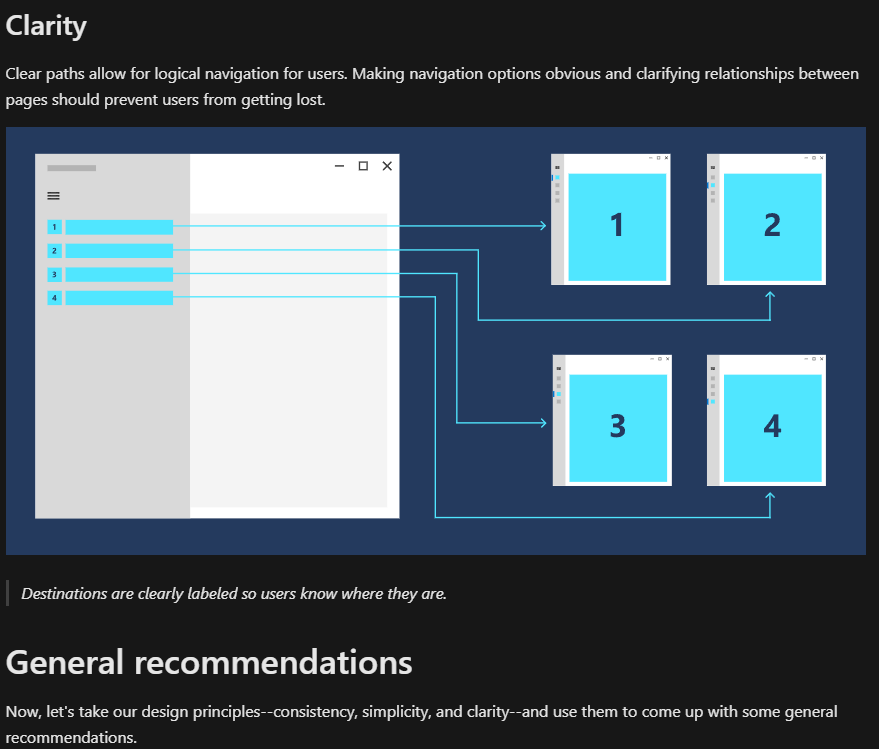
\includegraphics[width=1.0\textwidth]{gfx/design_system_ms.png}
   \caption{
      Ausschnitt aus der Dokumentation zum \textit{Fluent Design System}
   }
   \source{Microsoft}
   \label{fig:fluent}
\end{figure}


